

\section{L'analyse de Fourier, outil certes efficace mais insuffisant}

Les séries de Fourier (pour les signaux périodiques) et la transformée de Fourier (pour un signal quelconque) ont longtemps été les outils essentiels de l'analyse harmonique. \\
Le but de cette première partie est de présenter brièvement l'analyse de Fourier et de montrer ses limites.

\subsection{Le cas des signaux périodiques : l'utilisation des séries de Fourier}

Considérons $f$ fonction $2\pi$-périodique de classe $\mathcal{C}^{1}$ par morceaux. \\
Notons $S_{p}(f)$ la p-ième somme partielle de Fourier de $f$, ou p-ième somme partielle de la série de Fourier de $f$. \\
On a : $$ S_{p}(f)=\sum_{n=-p}^{p}c_{n}(f)e^{int} $$ en notation exponentielle ou bien $$ S_{p}(f)=\displaystyle\frac{a_{0}}{2}+\sum_{n=1}^{p}\left(a_{n}(f)\cos(nt)+b_{n}(f)\sin(nt)\right)$$ en notation trigonométrique ; \\
les $a_n$ et $b_n$ étant donnés par les relations 
$$ a_n=\displaystyle\frac{1}{\pi}\int_{0}^{2\pi}f(t)\cos(nt)\mathrm{d}t$$
$$ b_n=\displaystyle\frac{1}{\pi}\int_{0}^{2\pi}f(t)\sin(nt)\mathrm{d}t$$
\\
Le cours de mathématiques (plus particulièrement le théorème de Dirichlet) nous donne alors le résultat bien connu suivant, avec les hypothèses sur $f$ données plus haut : \\
\\
$f$ est somme de sa série de Fourier, ce qui se réécrit de la façon suivante :
$$\forall t\in\mathbb{R}, f(t)=\displaystyle\frac{a_{0}}{2}+\sum_{-\infty}^{+\infty}\left(a_{n}(f)\cos(nt)+b_{n}(f)\sin(nt)\right)$$
\\
On peut ainsi très facilement décomposer un signal périodique en une somme infinie de sinusoïdes. 

\pagebreak

\begin{figure}[!h]
\centering
<<<<<<< HEAD
\includegraphics[scale=0.2]{sinusoides.png}
=======
\includegraphics[scale=0.2]{images/sinusoides.png}
>>>>>>> d5245ec323332736ffd68589bb833e4bf5a5f8bb
\caption{Illustration du théorème de Fourier pour les signaux périodiques}
\end{figure}
Le signal "carré" en noir est la somme de toutes les sinusoïdes représentées, la sinusoïde rouge d'amplitude majeure étant appelée $\mathit{fondamentale}$ et les autres sinusoïdes étant les $\mathit{harmoniques}$. \\

 Bien évidemment, la plupart des signaux que l'on peut rencontrer sont non-périodiques et il est impossible d'obtenir une décomposition analogue à celle décrite ci-dessus. Dans le cas général et dans la limite de la possibilité de le faire, on effectue une transformation de Fourier.

\subsection{L'utilisation de la transformée de Fourier}

Il est nécessaire dans le cas plus général de fonctions/signaux non nécessairement périodiques de passer d'une écriture discrète en uneécriture en somme continue.
\\
Le cadre le plus naturel pour définir les transformations de Fourier est celui des fonctions $f$ intégrables\footnote{continues par morceaux et telles que $ \exists M \in \mathbb{R},\forall I\subset\mathbb{R}, \left|\int_{I}f(x)\right|\leq M$}. 
\\
On note alors traditionnellement $\mathcal{L}^{1}(\mathbb{R})$ l'ensemble des fonctions intégrables sur $\mathbb{R}$ et  $\mathcal{L}^{2}(\mathbb{R})$ l'ensemble des fonctions de carré intégrable sur $\mathbb{R}$.


\subsubsection{Définition de la transformation de Fourier}
 
On appelle transformation de Fourier l'application notée $\mathcal{F}$ qui, à toute fonction $f$ de  $\mathcal{L}^{1}(\mathbb{R})$, associe la fonction $\hat{f}$ telle que $\forall \omega \in \mathbb{R}$,$ \hat{f}(\omega)=\displaystyle{\frac{1}{\sqrt{2\pi}}\int_{-\infty}^{\infty}f(t)e^{-i\omega t}\:\mathrm{d}t}$
\\
$\hat{f}$ est appelée transformée de Fourier de $f$.
\\ \\
Notons toutefois que l'on peut donner plusieurs versions de définitions : nous avons ici choisi la définition plus "physicienne", car on y voit directement les paramètres de temps ($t$) en $s$ et de pulsation ($\omega$) en  $rad.s^{-1}$.
\\ \\
Notons aussi qu'il est possible de définir la transformée de Fourier pour des fonctions qui ne sont pas forcément dans $\mathcal{L}^{1}(\mathbb{R})$.
\\
\subsubsection{Propriétés de la transformation de Fourier} 
\begin{itemize}
\item $\mathcal{F}$ est clairement linéaire. \\
\item On peut montrer que $\mathcal{F}$ conserve la parité. \\
\item Propriété de translation : \\ Soit $a \in \mathbb{R}$ et $f\in \mathcal{L}^{1}(\mathbb{R})$ de la variable $t$. En effectuant le changement de variable $u=t-a$, on obtient la transformée de Fourier de la fonction d'expression $f(t-a)$. En effet : 
$$ \mathcal{F}[f(t-a)]=\displaystyle\int_{-\infty}^{\infty}f(t-a)e^{-i\omega t}\:\mathrm{d}t=\displaystyle e^{-i\omega a}\int_{-\infty}^{\infty}f(u)e^{-i \omega u}\:\mathrm{d}u=\displaystyle e^{-i\omega a}.\hat{f}(\omega) $$

\end{itemize}
 

\subsubsection{Transformée inverse}

On utilise les mêmes notations que précédemment.
Si $\hat{f}$ est elle-même une fonction intégrable, la formule dite de transformation de Fourier inverse, opération notée $\mathcal{F}^{-1}$ , et appliquée à $\hat{f}$, permet (sous conditions appropriéees) de retrouver $f$ :
$$ f(t)=\displaystyle{\frac{1}{\sqrt{2\pi}}\int_{-\infty}^{\infty}\hat{f}(\omega)e^{i\omega t}\:\mathrm{d}\omega}$$

Cette formule peut se démontrer facilement à partir de la formule sommatoire de Poisson.

\subsubsection{Ce qu'apporte la transformée de Fourier d'un signal}
Dans le cas général, la transformation de Fourier d'une fonction produit comme transformée une fonction $\hat{f}$ à valeurs complexes. Ainsi, on peut obtenir deux informations de cette transformée :

Le spectre d'amplitude : il s'agit du tracé du module de $\hat{f}(\omega)$ en fonction de la pulsation $\omega$.

Le spectre de phase :  il s'agit du tracé de l'argument de $\hat{f}(\omega)$ en fonction de la pulsation $\omega$.

Notons que l'on rencontre très souvent en traitement du signal les spectres en fréquence ; on passe de la pulsation $\omega$ à la fréquence par la relation de proportionnalité suivante : $f=\displaystyle \frac{1}{2\pi}\omega $.

On remarquera, comme le montre la figure ci-dessous, que le spectre d'amplitude d'un signal périodique est formé de traits verticaux.
\begin{figure}[!h]
\centering
<<<<<<< HEAD
\includegraphics[scale=0.4]{spectre.jpg}
=======
\includegraphics[scale=0.4]{images/spectre.jpg}
>>>>>>> d5245ec323332736ffd68589bb833e4bf5a5f8bb
\caption{Spectre de Fourier en fréquence d'un signal périodique}
\end{figure}

\subsubsection{Exemples de transformée de Fourier}

Facilement, on peut montrer que la transformée de Fourier d'une gaussienne\footnote{une fonction en $e^{\frac{-x^2}{2}}$.} est une gaussienne.
\begin{figure}[!h]
\centering
<<<<<<< HEAD
\includegraphics[scale=0.3]{gaussienne.png}
=======
\includegraphics[scale=0.3]{images/gaussienne.png}
>>>>>>> d5245ec323332736ffd68589bb833e4bf5a5f8bb
\caption{Allure d'une gaussienne}
\end{figure} \\ \\

Si on note $\Pi$ la fonction porte définie par 
$\forall t\in \left[-\frac{1}{2},\frac{1}{2} \right],\Pi(t)=1$ et $\forall t\in \mathbb{R} \backslash \left[-\frac{1}{2},\frac{1}{2} \right],\Pi(t)=0$, on obtient directement par intégration de l'exponentielle complexe et en tenant compte de la relation $\sin x = \displaystyle\frac{e^{ix}-e^{-ix}}{2i}$,
$\mathcal{F}(\Pi)(\omega) = \mathrm{sinc}(\frac{\omega}{2})$.  \footnote{la fonction sinc (sinus cardinal) est au premier sens mathématique la fonction définie sur $\mathbb{R}$* par sinc$(x)=\frac{\sin x}{x}$.} \\ La fonction étant réelle, son spectre de phase correspond à la fonction nulle et son spectre d'amplitude est le suivant : 
\begin{figure}[!h]
\centering
<<<<<<< HEAD
\includegraphics[scale=0.5]{sinc.jpg}
=======
\includegraphics[scale=0.5]{images/sinc.jpg}
>>>>>>> d5245ec323332736ffd68589bb833e4bf5a5f8bb
\caption{Spectre d'amplitude de la fonction $\Pi$}
\end{figure}


\subsubsection{Application de la transformation de Fourier}
En physique, la transformation de Fourier permet de déterminer le spectre d'un signal. 

En traitement d'images, on effectue des transformations de Fourier à deux dimensions : si $f$ est une fonction de $\mathbb{R}^2$ , sa transformée de Fourier est définie par : $$\hat{f}(u,v)=\int_{-\infty}^{\infty}\int_{-\infty}^{\infty}f(x,y).e^{-i(ux+vy)}\:\mathrm{d}x\:\mathrm{d}y$$
\\
On comprendra que la très grande majorité des signaux sont numériques et que les définitions mathématiques données jusqu'à présent ne sont pas adaptées au domaine du discret.

\subsection{Transformée de Fourier Discrète ou TFD et limites}

Bien évidemment, la transformée de Fourier telle qu'elle est utilisée dans un ordinateur (transformée de Fourier discrète (TFD)) possède une définition numérique différente de la définition mathématique donnée plus haut. 

\subsubsection{Définition}

Nous nous placerons dans le cas complexe (le cas réel en découle) sur un intervalle de temps fini correspondant à $N$ échantillons. Quand $N$ tend vers l'infini, on peut penser que l'on s'approche du cas continu mais il faut garder à l'esprit que la TFD suppose que le signal est périodique de période $N$.
\\ \\
Nous proposons la définition de la TFD d'un point de vue de l'algèbre linéaire, qui semble plus schématique :
\\
On définit ainsi la TFD comme un endomorphisme de $\mathbb{C}^N$ ayant pour matrice dans la base canonique de $\mathbb{C}^N$ la matrice S de terme général $s_{j,k}=\displaystyle{\frac{1}{N}e^{-2i\pi \frac{jk}{N}}}$, où $j,k\in \left\{0,1,...,N-1\right\}$. 
\\ \\
La TFD s'applique ainsi à des suites de longueur N (ou de période N) et on peut d'ailleurs remarquer que la TFD est périodique de période N.
\\ \\
On obtient ainsi, en l'appliquant à un vecteur $f=(f_0,...,f_{N-1})$ de $\mathbb{C}^N$ de matrice $F\in \mathcal{M}_{N,1}(\mathbb{C})$, le vecteur $g=(g_0,...,g_{N-1})$ de matrice $G=S$$\times$ $F$.
\\ On a clairement de la définition et du produit matriciel : 
$$\forall j\in \left\{0,1,...,N-1\right\}, g_j=\displaystyle\sum_{k=0}^{N-1}\displaystyle{\frac{1}{N}e^{-2i\pi \frac{jk}{N}}}f_k$$

En notant $W$ l'inverse de la racine $N$-ième de l'unité\footnote{$W=e^{\displaystyle-\frac{2i\pi}{N}}$}, il vient bien sûr : 
\begin{center}
\begin{equation}
$$$\forall j\in \left\{0,1,...,N-1\right\}, g_j=\displaystyle\sum_{k=0}^{N-1}W^{kj}f_k$$$
\end{equation}
\end{center}

\subsubsection{Des applications de la TFD}
La TFD a plusieurs applications, parmi lesquelles :  \\
\begin{enumerate}
\item L'analyse spectrale des signaux. \\ Il est intéressant pour un électronicien de mesurer par exemple la largeur de la bande de fréquence occupée par la transmission d'un signal, ceci grâce à une analyse spectrale. \\
\item La compression de données. \\  On applique sur les signaux la TFD pour réduire leur complexité. La suite des coefficients obtenus (en appliquant la formule ($1$)) est alors quantifiée avec des pas de quantification plus élevés pour les hautes fréquences, considérées comme négligeables pour la perception humaine. Le gain en compression vient de la réduction de précision de ces coefficients (voire leur suppression totale) : cela nécessite de ce fait moins de bits pour le codage.
\item La multiplication des grands nombres. \\ Certains des algorithmes les plus rapides (type FFT) pour la multiplication de grands nombres entiers sont fondés sur la TFD. 

\end{enumerate}

 Néanmoins, toutes ces applications nécessitent l'existence d'un algorithme rapide de calcul de la TFD et de son inverse. Les multiplications dans les cas où $N$ est petit sont "triviales", mais quand $N$ devient grand il est en effet indispensable d'utiliser un tel algorithme permettant de diminuer le nombre de multiplications. 


\subsubsection{Des limites à la Transformée de Fourier Discrète}
La TFD présente des limites considérables.
\\
On ne peut pas analyser un morceau de musique avec une TFD simple. En effet, on perdrait l'information temporelle.
Prenons par exemple deux signaux semblables :
\begin{enumerate}
\item un signal composé d'une sinusoïde à 100Hz pendant une seconde puis d'une sinusoïde à 200Hz pendant une seconde
\item  un second composé d'une sinusoïde à 200Hz pendant une seconde puis d'une sinusoïde à 100Hz pendant la seconde suivante.
\end{enumerate}

Leurs transformées de Fourier respectives seront identiques, ce qui est clair sur l'expression (1) (commutativité de l'addition).
\\
Par conséquent, la TFD n'est applicable que sur des signaux dont l'on sait que l'information fréquentielle est la même partout.
\\ \\
En outre, l'algorithme FFT nécessite que $N$ soit une puissance de 2 à cause de l'architecture récursive du programme. De plus, les algorithmes type FFT que l'on programme ne sont pas toujours efficaces au niveau de la mémoire et de la rapidité car on doit tenir compte des matrices et des nombres complexes que le logiciel de programmation ne connaît $\mathit{a\: priori}$ pas.
\\ \\ \\

On verra dans ce qui suit une transformation des fonctions/signaux plus performante, la transformation par les ondelettes qui est capable de détecter les portions du signal qui varient plus rapidement que d'autres.


